\documentclass{article}
%% to use a package, just delete the % character to enable the package in this document, only on the lines where there is a single % character (otherwise it won't compile)
%% to understand the utility of the package, please read the comment between \begin{comment} and \end{comment} right below the package you need
\usepackage[a4paper, total={6in, 8in}]{geometry} % for european user

%% for multiple lines comment in LaTeX
\usepackage{verbatim} % (won't compile if this line is deleted)
%% usage :
\begin{comment}
	Your multiple lines comment
\end{comment}


%% to include images
\usepackage{graphicx}
%% usage :
\begin{comment}
	\begin{figure}
		\centering %%(not necessary but it's prettier)
		\includegraphics[scale=(1 by default)]{path to the image/imageName.extension}
		%%if you want to put another image side to side, just add a line like the previous
		\caption{picture(s) in a nutshell} (not necessary but it's useful) (won't compile if missing)
	\end{figure}
\end{comment}


%% pour insérer des liens
%\usepackage{hyperref}
%% usage :
\begin{comment}
	\href{the complete link}{the display text}
	or if you want to show the complete link, just use 
	\url{the complete link}
\end{comment}


%% to display code easily (insert --shell-escape option when compile, otherwise, it won't compile)
%\usepackage{mint}
%% usage :
\begin{comment}
	- first, you have to have python3-pygments installed on your computer
	\begin{minted}{<language you choose>
		Your code
	\end{minted}
\end{comment}

%% to display code (for more informations, please see : https://texdoc.org/serve/listings.pdf/0)
%\usepackage{listings} 
%% usage :
\begin{comment}
	- listings package let you highly customize how you code will be displayed on the document
	- for simple display just do this :
	\lstdefinestyle{mystyle}{
		Your customizations
	}
	\begin{lstlisting}[language=<the language you'll use)
		Your code
	\end{lstlisting}
\end{comment}

%% to use maths and other sciences symbols (cf https://www.cmor-faculty.rice.edu/~heinken/latex/symbols.pdf) (
%\usepackage{amssymb,amsmath,amsfonts,extarrows}
%% usage : just type the backslash chararacter and the name of the symbol you want, depending of document on the the previous link

%% Have to find the goal of it
\usepackage{soul}
\let\oldemptyset\emptyset
\usepackage[T1]{fontenc}

%% won't compile if at least one of these three next line is deleted
%% but you can add nothing between the brackets to leave it blank
\author{Amnézic}
\date{}
\title{Linux}

\begin{document}
\maketitle
\newpage
%% not necessary
%% compile twice the first time to display table of content
\tableofcontents
\newpage

\section{Command Line Skills}
Le shell est un \textit{command line interpreter} et la CLI est une \textit{command line interface}.\newline
Le prompt est, initialement, sous cette forme là : username@systemName:$\$$pwd.\newline
Les commandes de bases : (on aura la commande avec ses principales options)
\begin{itemize}
    \item ls : liste les fichiers du dossier
    \item history : liste des commandes
        \begin{itemize}
            \item pour avoir accès à la n-ième commande : !n
            \item pour avoir accès à la dernière commande commençant par \textit{command} : !\textit{command}
        \end{itemize}
    \item cp
    \item rm
    \item type \textit{command} indique si \textit{command} est une commande interne (built-in) ou externe
    \item which \textit{command} indique où se trouve l'exécutable de \textit{command}
\end{itemize}

\noindent On peut créer des nouvells variables/commandes grâce aux alias : variable=value. Pour trouver la valeur d'une variable, on peut :
\begin{itemize}
    \item echo $\$$variable
    \item env | grep variable (ssi la variable est globale (faire export variable pour la mettre globale))
    \item unset variable pour supprimer la variable
\end{itemize}

La variable \textit{PATH} contient l'ensemble des dossiers contenant les exécutables des commandes. Pour ajouter un dossier à \textit{PATH}, il suffit de faire PATH=aNewPath:$\$$PATH .\newline

\noindent \underline{Display variables :}
\begin{itemize}
    \item rien ou double quote  " ": interprète les variables si ces dernières sont précédées par un $\$$
    \item single quote ' ': n'interprète jamais les variables mêmes si elles sont précédées par un $\$$
    \item si on ne veut pas que la variable avec le $\$$ soit interprétée, il faut rajouté un \ devant le $\$$
    \item back quote ` `: à n'utiliser qu'autour du nom seul de la variable qu'on veut afficher (pas de backslash ni de $\$$ nécessaire)
\end{itemize}

\noindent On peut exécuter plusieurs commandes à la suite grâce à :
\begin{itemize}
    \item ; : permet d'exécuter inconditionnellement les instructions les unes à la suite des autres
    \item $\&\&$: permet d'exécuter les instructions les unes à la suite des autres, mais si une commande renvoie une erreur, aucune des autres instructions à sa droite ne sera exécutée
    \item || : permet d'exécuter les instructions les une à la suite des autres jusqu'à ce qu'une commande ne renvoie pas d'erreur
\end{itemize}

\newpage
\section{Getting help}
Pour obtenir de l'aide sur une command, il suffit de faire : man \textit{command}. Les différentes sections des manuels sont :
\begin{enumerate}
    \item commandes générales, qui contient les informations suivantes :
        \begin{itemize}
            \item nom
            \item synopsis
            \item description
            \item options
            \item files
            \item author
            \item report bugs
            \item see also
            \item copyright
        \end{itemize}
    \item system calls
    \item lybrary calls
    \item special files
    \item file formats and conventions
    \item games
    \item miscellaneous
    \item system administration commands
    \item Kernel routines
\end{enumerate}

Pour :
\begin{itemize}
    \item connaitre quelles pages possède man \textit{command} : man -f \textit{command} (== whatis \textit{command})
    \item aller à une page n de man \textit{command} : man n \textit{command}
    \item chercher un manuel en rapport avec une action \textit{action} : man -k \textit{action} (== apropos \textit{action})
\end{itemize}

Il est aussi possible de retrouver cette documentation dans les dossier /usr/shar/doc ou usr/doc

\newpage
\section{Navigating the filesystem}
Pour se déplacer, on utilise la commande cd avec un chemin (absolu ou relatif). Pour savoir où on se trouve exactement, il suffit d'utiliser la commande \textit{pwd}.\newline
Pour lister le contenu d'un dossier, on utilise la commande \textit{ls} avec ces options là :
\begin{itemize}
    \item -l : long listing
    \item -a : affichage des fichiers cachés
    \item -r : ordre désalphabétique
    \item -h : human readable (taille des fichiers exprimés en o/ko/mo/go) 
    \item -d : listing de dossier(s) uniquement
    \item -R : listing récursif
    \item -S : trie par ordre alphabétique les fichiers
    \item -t : liste les fichiers du plus récemment modifié au moins récemment modifié
\end{itemize}


\newpage
\section{Managing files and directories}
Le file globbing est une manière d'englober un ensemble de combinaison de caractère bien précises. Ça se base sur le même principe que les RegEx avec les mêmes signes mais ne représentent pas forcément la même chose :
\begin{itemize}
    \item * : signifie qu'il y a 0 ou + caractères (!= RegEx car il indique n'importe quel caractère)
    \item ? : signifie qu'il y a exactement un caractère (??? comprend tous les mots qui possèdent exactement 3 lettres par exemple)
    \item \[ \] : représente un ensemble de caractère : \[az\] représente tous les mots qui ne contiennent qu'un 'a' ou qu'un 'z' alors que \[a-z\] représentent tous les mots qui ne contiennent qu'une lettre entre 'a' et 'z' inclus. Les rangées se basent sur le tableau ascii donc [a-Z] comprendra aussi les caractères entre 'z' et 'A' dans la table ascii (accessible via la commande ascii -d))
    \item ! ou $\hat{}$ : représente la négation
\end{itemize}

\newpage
\section{Working with text}
Pour lire un document comme si c'était un document papier (avec des pages donc), on peut utiliser la commande \textit{less}/\textit{more}. Si on veut rechercher un mot particulier, il suffit de taper : /\textit{mot} et se déplacer dans le texte en appuyant sur n.\newline
Pour afficher seulement une partie d'un document, on peut utiliser les deux commandes suivantes :
\begin{itemize}
    \item head (-n le nombre de ligne qu'on veut afficher) : affiche n (10 par défaut) lignes à partir du début du fichier
    \item tail (-n le nombre de ligne qu'on veut afficher) : affiche n (20 par défaut) lignes à partie de la fin du fichier 
\end{itemize}

Lorsqu'on travaille avec du texte, il est très pratique d'utiliser des pipes ( | ). Ça s'utilise comme ça :
\begin{quote}
    \textit{command1} | \textit{command2}
\end{quote}
Cette instruction va exécuter \textit{command1} et va renvoyer le résultat pour être utilisé par \textit{command2}.

Une notion importante est ce qu'on appelle les channels, il en existe 3 :
\begin{itemize}
    \item STDIN (0) : standard input, récupère les informations généralement via ce que l'utilisateur tape sur son clavier (on peut récupérer STDIN graĉe à '<')
    \item STDOUT (1) : standard output : ce qui est affiché dans la console et qui n'est pas une erreur (on peut renvoyer STDOUT grâce à '>')
    \item STDERR (2) : standard error : ce qui est affiché dans la console et qui est une erreur (on peut récupérer STDERR grâce à '2>')
\end{itemize}


Il peut être intéressant de trier les données que l'on a dans un fichier. Il existe deux commandes pour aider à sélectionner les bonnes donnés et les trier correctement :
\begin{itemize}
    \item sort :
        \begin{itemize}
            \item -n : permet de trier un ensemble de données numériques dans par ordre croissant
            \item -r : permet d'inverser le tri
            \item -k\textit{n} : permet de sélectionner uniquement la colonne \textit{n} (n peut être un ensemble) (commande à utiliser nécessairement avec -t)
            \item -t'\textit{délémiteur}' : indique à la machine que les différents champs sont séparés par \textit{délimiteur}
        \end{itemize}
    \item cut :
        \begin{itemize}
            \item -c\textit{n} : indique à la machine de ne garder que la colonne (un seul caractère)\textit{n} (n peut être un ensemble)
            \item -d'\textit{délimiteur}' : indique à la machine que les colonne seront séparées par des \textit{délimiteur} (à utiliser avec -f)
            \item -f\textit{n} : indique à la machine de ne garder que la section \textit{n} (n peut être un ensemble)
            \item --output-delimiter='\textit{char}' : indique à la machine de retourner le résultat avec des \textit{char} pour séparer les résultats
        \end{itemize}
\end{itemize}




\newpage
\section{Where data is stored}
Les informations sur les programmes en cours sont stockés dans le pseudo-dossier /proc. Les informations sur les composants électroniques sont stockés dans le dossier /dev ou /sys. Lorsque l'ordinateur démarre, il commence l'init process et lui assigne un PID (program ID) de 1, les suivant ont une valeur dans leur ordre d'exécution.\newline

On peut voir chaque programme en cours et ses enfants et récurivement avec la commande \textit{pstree} ou \textit{ps --forest}. Pour afficher l'ensemble des programmes en cours, on utilise la commande \textit{ps aux} ou \textit{ps -ef}. Pour voir les programmes en cours d'un autre utilisateur (si on fait partie du groupe root, on peut utiliser la commande suivante : \textit{ps -u <login>}.\newline

On peut aussi utiliser la commande \textit{top}:
\begin{itemize}
    \item permet de voir en temps réel certaines informations sur les programmes en cours
    \item il est affiché le load average sur une période (dans l'odre) : d'une minute, de 5 minutes et de 15 minutes. Si un des nombres est égal à 1, cela veut dire qu'il y a un coeur qui est complètement utilisé, mais pas nécessairement les autres
    \item il est affiché un PID qui est le dernier process à avoir été exécuté
    \item K PID : ferme le programme ayant pour PID PID
    \item R : ajuste la priorité d'un programme (-20<=R<=19)
\end{itemize}

\noindent Pour voir l'utilisation de la mémoire, on utilise la commande \textit{free} (-s n pour rafraichir toutes les n secondes (n=1 par défaut)).\newline

\newpage
\section{System and user security}
Pour changer d'utilisateur on utilise la commande su : 
\begin{itemize}
    \item su -  (root par défaut)
    \item su -l <login>
    \item su --login <login>
\end{itemize}

\noindent Ça va permettre de pouvoir effectuer des tâches que seul root peut exécuter avec la commande \textit{sudo <command>}.\newline
Le fichier /etc/passwd permet de trouver plusieurs informations sur tous les utilisateurs :
\begin{enumerate}
    \item le nom
    \item anciennement, le mot de passe (trouvable maintenant dans le fichier /etc/shadow)
    \item le user ID
    \item le primary group ID
    \item des commentaires
    \item chemin du home directory
    \item chemin vers le shell
\end{enumerate}
\noindent Le fichier /etc/shadow contient les informations sur les mots de passe des différents utilisateurs :
\begin{enumerate}
    \item le nom d'utilisateur
    \item le mot de passe : (plusieurs champs séparés par des $\$$)
        \begin{enumerate}
            \item un nombre (généralement 6)
            \item le sel
            \item le mot de passe hashé
        \end{enumerate}
    \item last change
    \item minimum de jours
    \item maximum de jours
    \item warning
    \item inactive
    \item temps avant expiration
\end{enumerate}

Pour avoir accès aux informations d'un utilisateur en particulier, on peut faire :
\begin{itemize}
    \item groupes : id <username>
    \item mot de passe : getent <type de données (ex: passwd)> <login>
\end{itemize}

\noindent Pour trouver les groupes d'un utilisateur, on peut aussi aller les chercher dans le fichier /etc/group : la première section contient le groupe primaire de l'utilisateur et la dernière l'ensemble des groupes dont fait partie l'utilisateur.\newline
Pour voir les utilisateurs qui sont en train d'utiliser la machine, on peut utiliser la commande \textit{who}.

\newpage
\section{Creating users and groups}
Commandes pour gérer les utilisateurs et les groupes :
\begin{itemize}
    \item groupadd <name>: permet de créer un nouveau groupe qui aura pour nom <name>
        \begin{itemize}
            \item -g n : associe le groupe <name> ou GID n
            \item -r : ??? (les GIDs jusqu'à 500 pour RedHat et jusqu'à 1000 pour Debian sont reservés au système)
        \end{itemize}
    \item groupmod <name> : permet de modifier des informations sur le groupe <name>
    \item groupdel <name> : permet de supprimer le groupe <name>
    \item useradd <username> : permet d'ajouter l'utilisateur <username>
    \item usermod <username> : permet de modifier des informations de <username>
    \item userdel <username> : permet de supprimer <username> (-r pour supprimer toutes ses données)
    \item passwd <username> : permet de changer le mot de passe de <username>
    \item chage [options] <username> : permet de modifier les options [options] de <username>
\end{itemize}

\newpage
\section{Ownership and permissions}
Pour connaitre toutes les informations d'un fichier, il faut utiliser l'option -l de ls. On aura alors quelquechose qui va ressembler à ça :
\begin{figure}
	\centering %%(not necessary but it's prettier)
	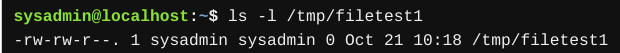
\includegraphics{Images/ll_example.png}
	%%\caption{picture(s) in a nutshell} (not necessary but it's useful) (won't compile if missing)
\end{figure}
On a dans l'ordre :
\begin{enumerate}
    \item si c'est un fichier classique (-), un dossier (d), un lien vers un autre dossier (l)
    \item les permissions, dans l'ordre, de l'owner, du groupe <group> et des autres
    \item le nom de l'owner
    \item le nom du groupe <group>
    \item d'autres trucs pas importants
    \item le nom du fichier
\end{enumerate}

\noindent Pour changer le groupe qui a le meilleur accès au fichier <file>, il suffit de faire \textit{chgrp <group> <file>} (-R si le fichier est un dossier).\newline
Pour changer le propriétaire d'un fichier, il faut exécuter la commande suivante : \textit{chown <newOwner> <file>}.

Pour changer les permissions de manière générale, on utilise la commande \textit{chmod} suivi soit de l'écriture complète (cf image ci dessous) ou de l'écriture numérique.
\begin{figure}[h]
    \centering
    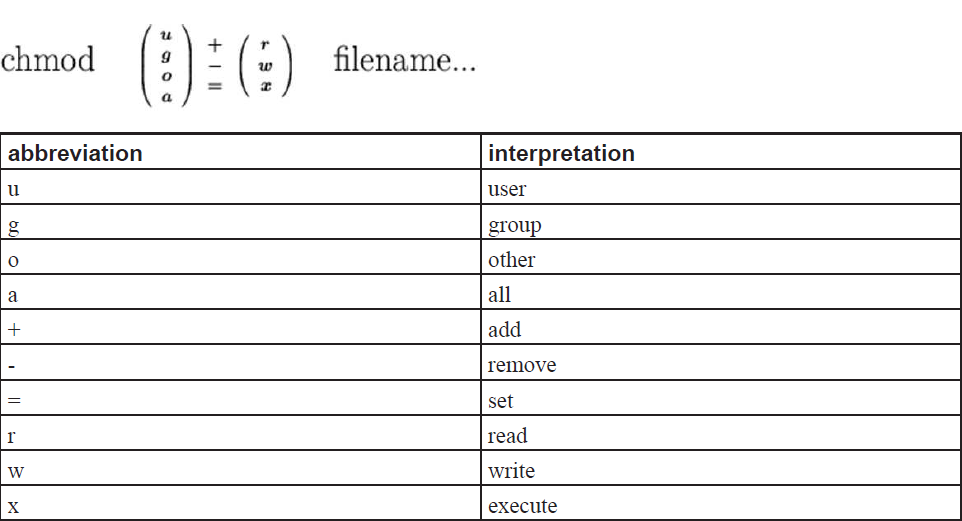
\includegraphics[scale=0.3]{Images/Permissions.png}
\end{figure}

Avec l'écriture numérique, il suffit de faire : \textit{chown value1value2value2 file} avec value1,2 et 3 la valeur des permissions pour, respectivement, l'owner, le group owner et les autres, sachant que :
\begin{itemize}
    \item r = 4
    \item w = 2
    \item x = 1
    \item on fait la somme des permissions de chaque "entité" et ça donner la valeur de value1, value2 et value3
\end{itemize}

\noindent Attention, pour que quelqu'un puisse modifier un document, il doit avoir la permission de modifier le document mais aussi de pouvoir aller jusqu'au dossier contenant le document à modifier.

\newpage
\section{Special directories and files}
\newpage
\section{Notes supplémentaires}
\end{document}
